\pagestyle{empty}

% Running Header
\noindent
\makebox[\textwidth][s]{%
  \textbf{\textsf{108}}\qquad \textbf{\textsf{CHƯƠNG 2}}\quad \textbullet\quad \textsf{Giới hạn và Đạo hàm}%
  \hfill%
}
\vspace{14pt}

\noindent
\begin{minipage}[t]{135pt}
  \vspace*{18pt}
  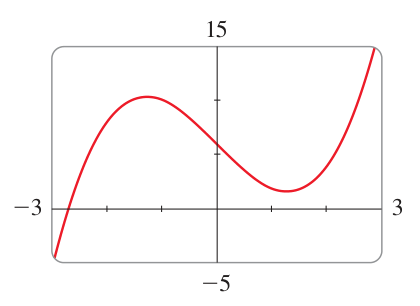
\includegraphics[width=\linewidth]{images/p0143_fig1.png}
  \vspace{2pt}
  \raggedright{\textbf{\textsf{\small HÌNH 7}}}\par

  \vspace{22pt}
  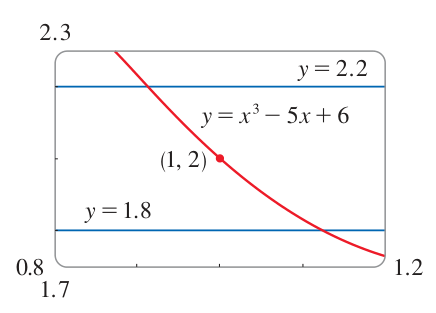
\includegraphics[width=\linewidth]{images/p0143_fig2.png}
  \vspace{2pt}
  \raggedright{\textbf{\textsf{\small HÌNH 8}}}\par
\end{minipage}%
\hspace{20pt}%
\begin{minipage}[t]{385pt}
  \setlength{\parindent}{14pt}
  \noindent
  Nói cách khác, tìm một số $\delta$ tương ứng với $\varepsilon = 0{,}2$ trong định nghĩa giới hạn đối với hàm số $f(x) = x^3 - 5x + 6$ với $a = 1$ và $L = 2$.

  \vspace{6pt}
  \noindent
  \textbf{\textsf{\color{stewartblue}LỜI GIẢI}}\quad Đồ thị của $f$ được thể hiện trong Hình 7; chúng ta quan tâm đến vùng lân cận điểm $(1, 2)$. Lưu ý rằng ta có thể viết lại bất đẳng thức
  \begin{align*}
    & |(x^3 - 5x + 6) - 2| < 0{,}2 \\
    \text{dưới dạng}\qquad & -0{,}2 < (x^3 - 5x + 6) - 2 < 0{,}2 \\
    \text{hay tương đương}\qquad & 1{,}8 < x^3 - 5x + 6 < 2{,}2
  \end{align*}
  Vì vậy chúng ta cần xác định các giá trị của $x$ sao cho đường cong $y = x^3 - 5x + 6$ nằm giữa hai đường nằm ngang $y = 1{,}8$ và $y = 2{,}2$. Do đó, chúng ta vẽ đồ thị các đường cong $y = x^3 - 5x + 6$, $y = 1{,}8$ và $y = 2{,}2$ gần điểm $(1, 2)$ trong Hình 8. Ta ước lượng hoành độ giao điểm của đường thẳng $y = 2{,}2$ và đường cong $y = x^3 - 5x + 6$ là khoảng $0{,}911$. Tương tự, $y = x^3 - 5x + 6$ cắt đường thẳng $y = 1{,}8$ khi $x \approx 1{,}124$. Vì vậy, làm tròn về phía $1$ để đảm bảo an toàn, ta có thể nói rằng
  \[
    \text{nếu}\qquad 0{,}92 < x < 1{,}12 \qquad\text{thì}\qquad 1{,}8 < x^3 - 5x + 6 < 2{,}2
  \]
  Khoảng $(0{,}92; 1{,}12)$ này không đối xứng qua $x = 1$. Khoảng cách từ $x = 1$ đến đầu mút bên trái là $1 - 0{,}92 = 0{,}08$ và khoảng cách đến đầu mút bên phải là $0{,}12$. Ta có thể chọn $\delta$ là số nhỏ hơn trong hai số này, nghĩa là $\delta = 0{,}08$. Khi đó ta có thể viết lại các bất đẳng thức theo khoảng cách như sau:
  \[
    \text{nếu}\qquad |x - 1| < 0{,}08 \qquad\text{thì}\qquad |(x^3 - 5x + 6) - 2| < 0{,}2
  \]
  Điều này chỉ nói lên rằng bằng cách giữ cho $x$ sai khác $1$ không quá $0{,}08$, chúng ta có thể giữ cho $f(x)$ sai khác $2$ không quá $0{,}2$.

  Mặc dù chúng ta đã chọn $\delta = 0{,}08$, bất kỳ giá trị dương nào nhỏ hơn của $\delta$ cũng đều thỏa mãn.\hfill\textcolor{stewartblue}{\rule{1.1ex}{1.1ex}}

  \vspace{6pt}
  Quy trình đồ thị được sử dụng trong Ví dụ 1 đem lại một minh họa trực quan cho định nghĩa với $\varepsilon = 0{,}2$, nhưng nó không \textit{chứng minh} rằng giới hạn bằng $2$. Một phép chứng minh phải cung cấp được một $\delta$ cho \textit{mọi} $\varepsilon$.

  Khi chứng minh các mệnh đề giới hạn, có thể hữu ích khi xem định nghĩa giới hạn như một thách thức. Trước tiên nó thách thức bạn với một số $\varepsilon$. Sau đó bạn phải tìm ra được một $\delta$ phù hợp. Bạn phải có khả năng làm điều này cho mọi $\varepsilon > 0$, chứ không chỉ cho một $\varepsilon$ cụ thể.

  Hãy hình dung một cuộc thi giữa hai người, A và B, và hãy tưởng tượng bản thân bạn là B. Người A quy định rằng số cố định $L$ phải được xấp xỉ bởi các giá trị của $f(x)$ trong phạm vi độ chính xác $\varepsilon$ (chẳng hạn, $0{,}01$). Người B sau đó đáp lại bằng cách tìm một số $\delta$ sao cho nếu $0 < |x - a| < \delta$, thì $|f(x) - L| < \varepsilon$. Sau đó A có thể trở nên khắt khe hơn và thách thức B với một giá trị $\varepsilon$ nhỏ hơn (chẳng hạn, $0{,}0001$). Một lần nữa B phải đáp ứng bằng cách tìm một $\delta$ tương ứng. Thông thường giá trị $\varepsilon$ càng nhỏ thì giá trị $\delta$ tương ứng cũng càng phải nhỏ. Nếu B luôn luôn thắng, bất kể A đưa ra $\varepsilon$ nhỏ đến mức nào, thì $\lim\limits_{x \to a} f(x) = L$.

  \vspace{7pt}
  \noindent
  \textbf{\textsf{\color{stewartblue}VÍ DỤ 2}}\quad Chứng minh rằng $\lim\limits_{x \to 3} (4x - 5) = 7$.

  \vspace{3pt}
  \noindent
  \textbf{\textsf{\color{stewartblue}LỜI GIẢI}}

  \vspace{1pt}
  \noindent
  \textbf{1.}\enspace \textit{Phân tích sơ bộ bài toán (đoán giá trị cho $\delta$).}\enspace Giả sử $\varepsilon$ là một số dương cho trước. Chúng ta muốn tìm một số $\delta$ sao cho
  \[
    \text{nếu}\qquad 0 < |x - 3| < \delta \qquad\text{thì}\qquad |(4x - 5) - 7| < \varepsilon
  \]
\end{minipage}

\vfill
\noindent
\begin{minipage}{\textwidth}
  \raggedright
  \fontsize{6.5}{8}\selectfont\color{black!60}
  Copyright 2021 Cengage Learning. All Rights Reserved. May not be copied, scanned, or duplicated, in whole or in part. WCN 02-200-203\par
  Editorial review has deemed that any suppressed content does not materially affect the overall learning experience. Cengage Learning reserves the right to remove additional content at any time if subsequent rights restrictions require it.
\end{minipage}
